\documentclass[aspectratio=169]{beamer}
\usepackage[utf8]{inputenc}
\usepackage{amsmath}
\usepackage{tikz}
\usepackage{pgfplots}
\usepackage{circuitikz}
\usetikzlibrary{decorations.markings}
\usetikzlibrary{arrows.meta}

\usetheme{NOVASBE}

\title[]{4509 - Bridging Mathematics}
\subtitle{Dynamic Optimization:\\Ramsey Cass Koopmans}
\author[P. Fagandini]{Paulo Fagandini}
\institute{}
\date{}

\newtheorem{defenition}{Definition}[section]
\newtheorem{proposition}{Conjecture}[section]

\begin{document}

\begin{frame}

    Consider a competitive economy with identical households that live forever and maximize the following utility function:
    
    \begin{align}
    \int_0^\infty \frac{c(t)^{1-\sigma}-1}{1-\sigma}e^{-\rho t}dt\label{eq_prob_0}
    \end{align} 
    
    where $\sigma>0$. At each point in time the household faces the following budget constraint:
    \[\dot{a}(t)=a(t)r(t)+y(t)-c(t)\]
    i.e. the instantaneous change in real assets held by the household is equal to the income minus their consumption. $y(t)$ represents an income unrelated to the assets held.
\end{frame}

\begin{frame}
    The household must choose paths for $c(t)$ and $a(t)$ in order to maximize \eqref{eq_prob_0}, given the initial wealth $a(0)$, the paths for the interest rate $r(t)$, and the non interest income $y(t)$.
\end{frame}

\begin{frame}
    The current-value Hamiltonian for the problem is:
    \begin{align}
        \mathcal{H}(t)=\frac{c(t)^{1-\sigma}}{1-\sigma}+\lambda(t)[a(t)r(t)+y(t)-c(t)]
    \end{align}
    
    Where the costate variable $\lambda(t)$ is the shadow price of wealth. Then the Hamiltonian again gives us the current flow of utility plus the utility value of the stock of assets that results of the current consumption decision. The Pontryagin conditions are:
    \begin{align}
        \frac{\partial\mathcal{H}(t)}{\partial c(t)}&=c(t)^{-\sigma}-\lambda(t)=0\quad\Rightarrow\nonumber\\
        c(t)^{-\sigma}&=\lambda(t)\label{eq:foc1}\\
        -\frac{\partial\mathcal{H}(t)}{\partial a(t)} &= -\lambda(t)r(t)=\dot{\lambda}(t)-\rho \lambda(t)\quad\Rightarrow\nonumber\\
        \frac{\dot{\lambda}(t)}{\lambda(t)}&=\rho-r(t)\label{eq:foc2}
    \end{align}
\end{frame}

\begin{frame}
    Taking derivatives with respect to time in \eqref{eq:foc1} we get \[-\sigma c(t)^{-\sigma-1}\dot{c}(t)=\dot{\lambda}(t)\Rightarrow -\sigma \frac{\dot{c}(t)}{c(t)}=\frac{\dot{\lambda}(t)}{c(t)^{-\sigma}}=\frac{\dot{\lambda}(t)}{\lambda(t)}\]
    So we have the condition \[-\sigma \frac{\dot{c}(t)}{c(t)}=\frac{\dot{\lambda}(t)}{\lambda(t)}\] that we can replace in \eqref{eq:foc2} to get
    \begin{align}
        \frac{\dot{c}(t)}{c(t)}=\frac{r(t)-\rho}{\sigma}
    \end{align}
\end{frame}

\begin{frame}

    Together with the transversality conditions:
    
    \begin{align}
        \lim_{t\rightarrow\infty} a(t)e^{-\rho t}\geq 0 \quad\text{and}\quad \lim_{t\rightarrow\infty} a(t)\lambda(t)e^{-\rho t}=0
    \end{align}

    We have the system that describes the optimal path for consumption and asset holdings:
    
    \begin{align*}
        \dot{a}(t)&=a(t)r(t)+y(t)-c(t)\\
        \frac{\dot{c}(t)}{c(t)}&=\frac{r(t)-\rho}{\sigma}
    \end{align*}
    for given paths of income and the interest rate.
\end{frame}

\begin{frame}
    Integrating for the flow budget constraint:
    \begin{align*}
        \dot{a}(t)-a(t)r(t)=y(t)-c(t)
    \end{align*}
    Multiply in both sides by $e^{-\int_0^t r(s)ds}$
    \begin{align*}
        e^{-\int_0^t r(s)ds}[\dot{a}(t)-a(t)r(t)]=e^{-\int_0^t r(s)ds}[y(t)-c(t)]
    \end{align*}
    And note that the left hand side is the derivative of \(a(t)e^{-\int_0^t r(s)ds}\) with respect to $t$, so we can rewrite the previous equation as:
    \begin{align*}
        \frac{d}{dt}\left[a(t)e^{-\int_0^t r(s)ds}\right]=e^{-\int_0^t r(s)ds}[y(t)-c(t)]
    \end{align*}
    And integrating in both sides we obtain,
\end{frame}

\begin{frame}
    \begin{align*}
        \int_0^t \frac{d}{dt}\left[a(s)e^{-\int_0^s r(s)ds}\right]ds = \int_0^t e^{-\int_0^s r(\phi)d\phi}(y(s)-c(s))ds\\
        a(s)e^{-\int_0^s r(\phi)d\phi}\bigg\vert_{0}^{t}=\int_0^t e^{-\int_0^s r(\phi)d\phi} (y(s)-c(s))ds\\
        a(t)e^{-\int_0^t r(s)ds}=a(0)+\int_0^t(y(s)-c(s))e^{-\int_0^s r(\phi)d\phi}ds
    \end{align*}
    Note the intuition of the equation: The value at time 0 of the present assets is equal to the initial assets plus the discounted value of accumulated savings.
\end{frame}

\begin{frame}
    And for the consumption path:
    \begin{align*}
        \ln(c(t))-\ln(c(0))&=\int_0^t \frac{r(s)-\rho}{\sigma}ds\\
        c(t)&=c(0)e^{\frac{1}{\sigma}\int_0^t r(s)-\rho ds}
    \end{align*}
\end{frame}

\begin{frame}
    We have the following equations at our disposal:
    \begin{align}
        0&\leq\lim_{t\rightarrow\infty} a(t)e^{-\rho t}\label{eq:1transv}\\
        0&=\lim_{t\rightarrow\infty} a(t)\lambda(t)e^{-\rho t}\label{eq:2transv}\\
        c(t)&=c(0)e^{\frac{1}{\sigma}\int_0^t r(s)-\rho ds}\label{eq:fin_con}\\
        a(t)e^{-\int_0^t r(s)ds}&=a(0)+\int_0^t(y(s)-c(s))e^{-\int_0^s r(\phi)d\phi}ds\label{eq:fin_as}
    \end{align}
    
    The ``economics'' of the transversality condition in \eqref{eq:1transv} is that at present value, we cannot leave debt in the \emph{end}.
\end{frame}

\begin{frame}
    
    Take \eqref{eq:1transv} and \eqref{eq:fin_as}:
    \[\lim_{t\rightarrow\infty}\left(a(0)+\int_0^t e^{-\int_0^sr(\phi)d\phi} (y(s)-c(s))ds\right)e^{-\int_0^tr(s)ds-\rho t}\geq 0\]
    
    This implies that:
    \[a(0)+\underbrace{\int_0^\infty e^{-\int_0^sr(\phi)d\phi}y(s)ds}_{Y_0} - \underbrace{\int_0^\infty e^{-\int_0^sr(\phi)d\phi}c(s)ds}_{PVC_0}\geq0\]
    \begin{itemize}
        \item $a_0$ is the initial wealth
        \item $Y_0$ is the present value (at $t=0$) of the income stream.
        \item $PVC_0$ is the present value (at $t=0$) of the consumption stream.
    \end{itemize}
\end{frame}

\begin{frame}
    Rewrite the transversality constraint as:
    \[PVC_0\leq a(0)+Y_0\]
    i.e. the present value (at $t=0$) of the lifetime consumption, cannot exceed total wealth! Indeed, this constraint will hold in equality, otherwise there was money left on the table...
\end{frame}

\begin{frame}
    Now take the second transversality constraint:
    {\scriptsize
    \[\lim_{t\rightarrow\infty}\left(a(0)+\int_0^t e^{-\int_0^sr(\phi)d\phi} (y(s)-c(s))ds\right)e^{\int_0^tr(s)ds-\rho t}\underbrace{C(0)^{-\sigma}e^{-\int_0^t(r(s)-\rho)ds}}_{\lambda(t)=c(t)^{-\sigma}}= 0\]
    }
    
    And noting that \[-\int_0^t(r(s)-\rho)ds=\rho t - \int_0^t r(s)ds\] and $c(0)\neq 0$
    
    We can simplify the previous expression to:
    {\small
    \begin{align}
        \left(a(0)+\int_0^\infty e^{-\int_0^s r(\phi)d\phi}y(s)ds\right)-\int_0^\infty e^{-\int_0^s r(\phi)d\phi}c(s)ds=0
    \end{align}
    } or
    \[a(0)+Y_0=PVC_0\]
\end{frame}

\begin{frame}
Substituting $c(t)=c(0)e^{\frac{1}{\sigma}\int_0^t (r(s)-\rho) ds}$ into $PVC_0$ we get:
\begin{align*}
    \int_0^\infty e^{\frac{1}{\sigma}\int_0^s (r(\phi)-\rho)d\phi-\int_0^s r(\phi)d\phi}c(0)ds = a(0)+Y_0
\end{align*}
    From where we can get $c(0)$
    
    \begin{align}
        c(0)=\frac{a(0)+Y_0}{\int_0^\infty e^{\frac{1}{\sigma}\int_0^s (r(\phi)-\rho)d\phi-\int_0^s r(\phi)d\phi}ds}
    \end{align}
    
    So consumption (at $t=0$, and therefore for any $t$) depends on the whole time path of income and interest rates!
\end{frame}

\begin{frame}

    Note that so far, $y(t)$ and $r(t)$ have been assumed exogenous. Let's put our consumer within context.

\end{frame}

\begin{frame}

    Assume that the firm's technology is described by a neoclassical production function with constant returns to scale and labor-augmenting exogenous technical change, $i.e.$ \[Y(t)=F(K(t),Z(t)L(t))=Z(t)L(t)f(k(t))\] where \[k(t)=\frac{K(t)}{Z(t)L(t)}\quad\text{and}\quad f(k(t))\equiv F(k(t),1)\] and technology progresses at a rate $g$, $i.e.$ \[\frac{\dot{Z}(t)}{Z(t)}=g\]

\end{frame}

\begin{frame}
    
    Firms rent capital and labor in competitive markets at their equilibrium prices, given by the marginal products of capital and labor:
    \begin{align}
        r(t) &= f'(k(t))-\delta\\
        w(t) &= w(k(t)) = f(k(t))-f'(k(t))k(t)
    \end{align}
    Assume population is constant and equal to $1$. Agents have no preference for leisure, so they offer all their time inelastically at every time, so $L(t)=1$ $\forall t$.
\end{frame}

\begin{frame}
    The government taxes labor and net capital incomes at \emph{ad-valorem} rates $\tau_w$ and $\tau_r$, and with those taxes makes \emph{lump-sum} transfers to individuals of $P(t)$, and destines $X(t)$ units of output to provide public goods. Assume the government must have balanced accounts and that $x$ and $p$ are constant over time. \footnote{In general lower caps means per efficiency unit of labor.} The government's budget constraint is therefore defined by:
    \begin{align}
        \tau_r\underbrace{[f'(k(t))-\delta]}_{r(t)}k(t)+\tau_w w(k(t))=x+p
    \end{align}
\end{frame}

\begin{frame}
    Substituting $r(t)$ in the differential equation that describes the consumption's trajectory we obtain:
    \begin{align}
        \frac{\dot{c}(t)}{c(t)}=\frac{(1-\tau_r)[f'(k(t))-\delta]-\rho}{\sigma}
    \end{align}
    And the non-interest income of an agent is given by:
    \begin{align}
        y(t)=(1-\tau_w)Z(t)w(k(t))+Z(t)p
    \end{align}
\end{frame}

\begin{frame}
    Recall that there are no assets other than capital; therefore, $a(t)=Z(t)k(t)=\kappa(t)$,\footnote{$\kappa(t)$ is the capital \textit{per capita}.} so the flow budget constraint becomes:
    {\scriptsize
    \begin{align*}
        \dot{\kappa}(t)&=(1-\tau_r)[f'(k(t))-\delta]Z(t)k(t)+(1-\tau_w)Z(t)w(k(t))+pZ(t)-c(t)
    \end{align*}
    }
    And rearranging we obtain:
    {\tiny
    \begin{align*}
        \dot{\kappa}(t)=Z(t)[\underbrace{f'(k(t))k(t)+w(k(t))}_{f(k(t))}]-\delta\kappa(t)-c(t)-Z(t)\{\underbrace{\tau_r[f'(k(t))-\delta]k(t)+\tau_w w(k(t))-p}_{x}\}
    \end{align*}
    }
    \begin{align}
        \dot{\kappa(t)}=Z(t)f(k(t))-\delta\kappa(t)-c(t)-Z(t)x
    \end{align}
    Divide by $\kappa(t)$ on both sides to get
    \begin{align}
        \frac{\dot{\kappa}(t)}{\kappa(t)} = \frac{Z(t)f(k(t))}{\kappa(t)}-\delta-\frac{c(t)}{\kappa(t)}-\frac{Z(t)x}{\kappa(t)}
    \end{align}
\end{frame}

\begin{frame}

    And recalling that $\kappa(t)=Z(t)k(t)$ we have:
    \begin{align*}
        \frac{\dot{\kappa}(t)}{\kappa(t)} = \frac{Z(t)f(k(t))}{Z(t)k(t)}-\delta-\frac{c(t)}{Z(t)k(t)}-\frac{Z(t)x}{Z(t)k(t)}
    \end{align*}
    or,
    \begin{align*}
        \frac{\dot{\kappa}(t)}{\kappa(t)} = \frac{f(k(t))}{k(t)}-\delta-\frac{c(t)}{Z(t)k(t)}-\frac{x}{k(t)}
    \end{align*}
\end{frame}

\begin{frame}
    The system, in\textit{ per capita terms} is:
    \begin{align}
        \frac{\dot{c}(t)}{c(t)}&=\frac{(1-\tau_r)[f'(k(t))-\delta]-\rho}{\sigma}\\
        \frac{\dot{\kappa}(t)}{\kappa(t)} &= \frac{f(k(t))}{k(t)}-\delta-\frac{c(t)}{Z(t)k(t)}-\frac{x}{k(t)}
    \end{align}
    
    With exogenous growth of productivity ($Z(t)$) consumption \textit{per capita} (and the stock of capital \textit{per capita}) growths without bounds... we have no steady state. We need to write the system in terms of per unit of efficiency labor instead of \emph{per capita}.
\end{frame}

\begin{frame}

Let \[\zeta(t)=\frac{c(t)}{Z(t)}\], then \[\dot{\zeta}=\frac{\dot{c}(t)Z(t)-c(t)\dot{Z}(t)}{Z(t)^2}=\frac{\dot{c}(t)}{Z(t)}-\zeta(t)g\] and 
\[\dot{\zeta}=\frac{\dot{c}(t)}{Z(t)}\frac{c(t)}{c(t)}-\zeta(t)g=\frac{\dot{c}(t)}{c(t)}\zeta(t)-\zeta(t)g\]
Finally we have \[\frac{\dot{c}(t)}{c(t)}=\frac{\dot{\zeta}(t)}{\zeta(t)}+g\]

Which we can replace back to our system.
\end{frame}

\begin{frame}
    Equivalently, we have \[k(t)=\frac{\kappa(t)}{Z(t)}\] and, \[\dot{k}(t)=\frac{\dot{\kappa}(t)Z(t)-\kappa(t)\dot{Z}(t)}{Z(t)^2}=\frac{\dot{\kappa}(t)}{Z(t)}-\frac{\kappa(t)}{Z(t)}g\]
    further,
    \[\dot{k}(t)=\frac{\dot{\kappa}(t)}{Z(t)}\frac{\kappa(t)}{\kappa(t)}-k(t)g=\frac{\dot{\kappa}(t)}{\kappa(t)}k(t)-k(t)g\]
    Finally we have
    \[\frac{\dot{\kappa}(t)}{\kappa(t)}=\frac{\dot{k}(t)}{k(t)}+g\]
    Which we can also replace back in our system,
\end{frame}


\begin{frame}
    \begin{align}
        \frac{\dot{\zeta}(t)}{\zeta(t)}&=\frac{(1-\tau_r)[f'(k(t))-\delta]-\rho}{\sigma}-g\\
        \frac{\dot{k}(t)}{k(t)} &= \frac{f(k(t))}{k(t)}-\delta-\frac{\zeta(t)}{k(t)}-\frac{x}{k(t)}-g
    \end{align}
    Which can be rewritten as:
    \begin{align}
        \dot{\zeta}(t) &= \left(\frac{(1-\tau_r)[f'(k(t))-\delta]-\rho}{\sigma}-g\right)\zeta(t)\\
        \dot{k}(t)&=f(k(t))-(g+\delta)k(t)-\zeta(t)-x
    \end{align}
    
    Let's look at the phase diagram...
\end{frame}

\begin{frame}
    Note that \[\dot{\zeta}(t)\geq 0 \Leftrightarrow f'(k(t))\geq \frac{g\sigma+\rho}{1-\tau_r}+\delta \] and
    \[\dot{k}(t)\geq0\Leftrightarrow \zeta(t)\leq f(k(t))-(g+\delta)k(t)-x\]
    
    Assume further than $f(0)=0$, $f'(0)=\infty$, and $f'(\infty)=0$. Further, let $x$ be small enough for the region $\dot{k}(t)=0$ be in the region with positive values of $\zeta(t)$.
    
    These conditions ensure the existence of a unique steady state in terms of per unit of efficiency labor $(k^*,\zeta^*)$.
\end{frame}

\begin{frame}
    \begin{center}
        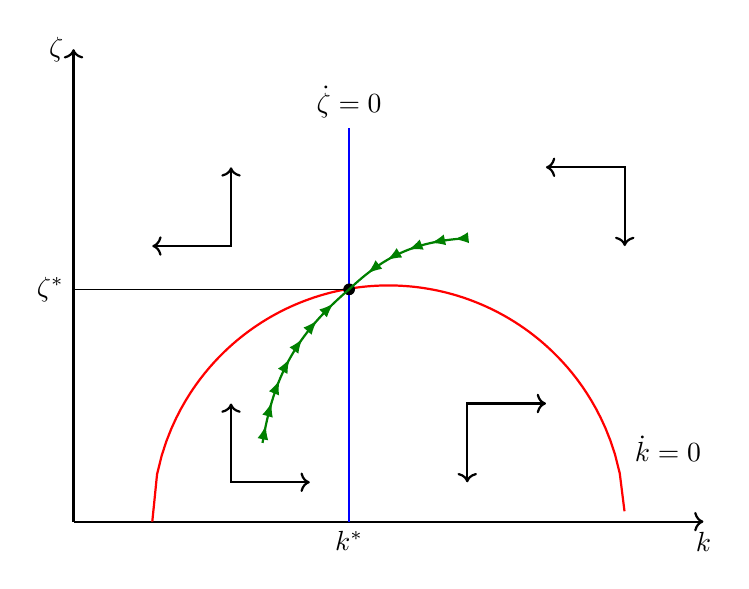
\begin{tikzpicture}[
                scale=2,
                decoration={
                    markings, 
                    mark= between positions 0.1 and 0.9 step 3mm with {\arrow{latex}} %{\arrowreversed{latex}}
                }
                ]
            \draw[thick,->] (0,0)--(4,0)node[below]{$k$};
            \draw[thick,->] (0,0)--(0,3)node[left]{$\zeta$};
            \draw[thick,red,domain=0.5:3.5,variable=\x,samples=100] plot (\x,{(2.25-(\x-2)^2)^(0.5)})node[above right,yshift=0.5cm,black]{$\dot{k}=0$};
            \draw[thick,blue] (1.75,0) -- (1.75,2.5)node[above,black]{$\dot{\zeta}=0$};
            
            \onslide<2->{
                \draw[] (1.75,0)node[below]{$k^*$};
                \draw[] (0,1.475)node[left]{$\zeta^*$}--(1.75,1.475)node[circle,fill,inner sep=1.5pt]{};
            }
            
            \onslide<3->{
                \draw[<->,thick] (1,0.75)--(1,0.25)--(1.5,0.25);
                \draw[<->,thick] (1,2.25)--(1,1.75)--(0.5,1.75);
                \draw[<->,thick] (3.5,1.75)--(3.5,2.25)--(3,2.25);
                \draw[<->,thick] (2.5,0.25)--(2.5,0.75)--(3,0.75);
            }
            
            \onslide<4->{
                \draw[green!50!black,thick,postaction={decorate}] (1.2,0.5) to[bend left=20](1.75,1.475);
                \draw[green!50!black,thick,postaction={decorate}] (2.5,1.8) to[bend right=20](1.75,1.475);
            }
            
        \end{tikzpicture}
    \end{center}
\end{frame}

\begin{frame}
    Let's verify this is a saddle path:
    \begin{align*}
        J(\zeta^*,k^*)=\begin{bmatrix}\frac{\partial\dot{\zeta}}{\partial \zeta}(\zeta^*,k^*)&\frac{\partial\dot{\zeta}}{\partial k}(\zeta^*,k^*)\\ \frac{\partial\dot{k}}{\partial \zeta}(\zeta^*,k^*)&\frac{\partial\dot{k}}{\partial k}(\zeta^*,k^*)\end{bmatrix}=\begin{bmatrix}0&\frac{\zeta^*(1-\tau_r)f''(k^*)}{\sigma}\\-1&f'(k^*)-g-\delta\end{bmatrix}
    \end{align*}
    
    Using the fact that the determinant of a matrix is equal to the product of the eigenvalues, we have that
    \[\lambda_1\lambda_2=\frac{\zeta^*(1-\tau_r)f''(k^*)}{\sigma}\]
    Noting that $f''<0$, we have that the eigenvalues have opposite signs, and therefore we are in the presence of a saddle.
\end{frame}

\end{document}
